\documentclass[11pt, openany]{memoir}
\usepackage[utf8]{inputenc}
\usepackage[T1]{fontenc}
\usepackage{amsfonts}
\usepackage{amsmath}
\usepackage{amsthm}
\usepackage[hidelinks]{hyperref}
\usepackage{titlesec} %title formatting
\usepackage{color}
\usepackage[textwidth=5.5in,textheight=9.2in,centering,a4paper]{geometry}
\usepackage{nth}
\usepackage{quiver}
\usepackage{marginnote}
\usepackage{tikz}
\usepackage{mathtools} % \coloneqq
%\usepackage{stix2}
\usepackage{newtxtext}
\usepackage{newtxmath}

\usetikzlibrary{patterns} 

\setlength{\abovedisplayskip}{0pt}
\setlength{\belowdisplayskip}{0pt}
\setlength{\abovedisplayshortskip}{0pt}
\setlength{\belowdisplayshortskip}{0pt}

\setlength{\parindent}{0pt}

\hypersetup{
    colorlinks,
    citecolor=black,
    filecolor=black,
    linkcolor=black,
    urlcolor=black
}

\renewcommand{\Top}{\mathsf{Top}}
\newcommand{\Set}{\mathsf{Set}}
\newcommand{\Disc}{\mathsf{Disc}}
\newcommand{\CoDisc}{\mathsf{CoDisc}}
\newcommand{\Hom}{\mathsf{Hom}}
\newcommand{\R}{\mathbb{R}}
\newcommand{\Z}{\mathbb{Z}}
\newcommand{\OO}{\mathcal{O}}
\DeclareMathOperator{\Spec}{Spec}


\theoremstyle{definition}
\newtheorem{proposition}{Proposition}
\newtheorem{definition}{Definition}
\newtheorem{construction}{Construction}
\newtheorem{example}{Example}
\newtheorem{lemma}{Lemma}
\newtheorem{theorem}{Theorem}

\makeatletter
\newcommand{\colim@}[2]{%
  \vtop{\m@th\ialign{##\cr
    \hfil$#1\operator@font lim$\hfil\cr
    \noalign{\nointerlineskip\kern1.5\ex@}#2\cr
    \noalign{\nointerlineskip\kern-\ex@}\cr}}%
}
\newcommand{\colim}{%
  \mathop{\mathpalette\colim@{\rightarrowfill@\textstyle}}\nmlimits@
}
\newcommand{\op}{
  o\kern-0.10em p
}
\newcommand{\Op}{
  O\kern-0.10em p
}
\newcommand{\Ext}{
  E\kern-0.06em x\kern-0.02em t
}
\newcommand{\indexset}[2]{
  \, #1\, \in \, #2
}
\makeatother

% title formatting
\definecolor{gray75}{gray}{0.75}
\titleformat{\chapter}[hang]{\Huge\bfseries}{\thechapter\hspace{20pt}\textcolor{gray75}{|}\hspace{20pt}}{0pt}{\Huge\bfseries}
%\renewcommand{\chapterheadstartvskip}{\vspace*{-2\baselineskip}}
\titlespacing*{\chapter}{0pt}{-2\baselineskip}{1em}

\begin{document}
  \nocite{*}

  \chapter*{Abstract}
  We develop the basic geometry behind the \'etale topos of a scheme. First we develop the notion of \'etale morphism and show how they behave like local homeomorphisms. We then apply this theory to construct the \'etale fundamental group of a scheme. Finally we consider sheaves on the \'etale site of a scheme and show how the category of sheaves on a scheme admits an internal logic.


  \begin{KeepFromToc} 
  \tableofcontents
  \end{KeepFromToc} 

  \chapter{Introduction}
  \subsection{Introduction}
The goal of this text is to give an overview of the geometry behind \'etale cohomology.
\section{Reminder on Schemes}

The basic building blocks of algebraic geometry are affine schemes. An affine scheme $\Spec(A)$ is a geometric object constructed out of the prime spectrum 
\[
  \{p \subseteq A \mid p \text{ prime ideal}\}
\]
of a commutative ring $A$. This set is equipped with the Zariski topology, which has a basis given by sets of the form 
\begin{align*}
  D_f &= \{ p \in \Spec(A) \mid (f) \not \subseteq p \} \\
      &= \{ p \in \Spec(A) \mid f(p) \neq 0\} .
\end{align*}
\begin{definition}
    The \textit{Zariski topology} on $\Spec(R)$ consists of open sets of the form $D_I = \{ p \in \Spec(A) \mid I \not \subset (p)\}$. The closed sets are of the form
    \begin{align*}
        V_I &= \{ p \in \Spec(A) \mid (f) \subseteq p \} \\
            &= \{ p \in \Spec(A) \mid f(p) = 0\},
    \end{align*}
    the \textit{vanishing set} or \textit{zero locus} of $f$. 
\end{definition}

Here $f(p)$ denotes the image of $f$ under the quotient map $A \to A/p$. This notation indicates that we interpret the elements $f \in A$ as functions on the space $\Spec(A)$. Since $f(p) \neq 0$ for all $p \in D_f$, we view the the ring $A[1/f]$ as the ring of rational functions defined on $D_f$. It consists of elements of the form 
\[
  \biggl\{ \frac{g}{f^k} \mid g \in A, k \in \N \biggr\}.
\]
The assingment $D_f \to A[1/f]$ extends to a sheaf $\Sh{O}_{\Spec{A}}: \Spec(A) \to \mathsf{Ring}$, called the \textit{structure sheaf of $\Spec(A)$}. We obtain a fully faithful functor
\[
\Spec : \text{CRing} \to LRS
\]
from the category of commutative rings to the category of locally ringed spaces. An affine schemes is a locally ringed space isomorphic to $\Spec(R)$ for some ring $R$.

\begin{definition}
  A \textit{scheme} is a locally ringed space $X$ such that there is a covering $\{U_i\}_{i \in I}$ of $X$ such that each $U_i$ is isomorphic to an affine scheme $\Spec(A_i)$ for some ring $A_i$.
\end{definition}

\subsection{Motivation for Cohomology}
One of the most important invariants of schemes is \'etale cohomology.  Cohomology is an important invariant in geometry and topology which associates to each space $X$ a sequence of abelian groups $H^i(X)$, $i \ge 0$, the so-called cohomology groups of $X$. For each map $f: X \to Y$ of spaces there are homomorphisms $f^*: H^i(Y) \to H^i(X)$. Moreover there are so called coboundary morphisms $\partial^i : H^i \to H^i+1$ for each $i \ge 0$. In other words, 
\begin{definition}
    a \textit{cohomology theory} for
\end{definition}
We can deduce many interesting properties of spaces from their cohomology groups and the associated homomorphisms.

The first example of cohomology one usually encounters first is singular cohomology. This cohomology theory provides a rigorous way for counting ``holes'' in a topological space.  For instance, the circle $S^1$ has 1 one-dimensional hole while the torus $T^2$ has 2. The sphere $S^2$ has 1 two-dimensional hole but no one-dimensional holes, in symbols 
\footnote{$\Z$ appears here because it is the free group on one generator.}
\begin{align*}
  H^1_{sing}(S^1) \cong \Z,\quad &H^1_{sing}(T^2) \cong \Z \oplus \Z,\\
  H^1_{sing}(S^2) \cong  0,\quad &H^2_{sing}(S^2) \cong \Z.
\end{align*}
One very general approach to cohomology is to use sheaves on a topological space as ``coefficients''. For any space $X$ and any sheaf $\Sh{F}$ on $X$ we can define $H^i(X, \Sh{F})$. Many examples of cohomology turn out to stem from the cohomology of a particular sheaf. For example, if $X$ is a locally contractible space, the singular cohomology $H_{\text{sing}}^i(X)$ of $X$ is isomorphic to the sheaf cohomology $H^i(X, \Z_X)$ of the constant sheaf $\Z_X$ on $X$.

One of the main motivations for \'etale cohomology is that one would like a replacment for singular cohomology for schemes. There are a number of obstacles:
\begin{proposition}\label{scheme_contractible}
    An irreducible scheme is contractible.
\end{proposition}
\begin{proof}
  Define a map $f: X \times I \to X$  by $f(x,0) = x$ and $f(x,t) = \eta$ for $t > 0$. This is a contraction of $X$ onto the point $\eta$, so. the singular cohomology of $X$ is identically 0.
\end{proof}
\begin{proposition}
  $H^i(X, \Sh{F})$ is 0 for any sheaf on an irreducible topological space.
\end{proposition}
\begin{proof}
    See section TODO.
\end{proof}

\subsection{Fundamental groups}
Another important invariant of spaces is the fundamental group. The fundamental group of a pointed topological space $(X,x)$, denoted by $\pi_1(X,x)$ may be defined in two equivalent ways:
\begin{construction}[the fundamental group via paths]
    A loop with base point $x$ is a map $\gamma : [0,1] \to X$ such that $\gamma(0) = \gamma(1) = x$. The homotopy class of $\gamma $ is denoted by $[\gamma]$. Define a composition operation by concatenation: $[\gamma] \circ [\eta] = [\gamma \circ \eta]$, where $\gamma \circ \eta$ is defined to be the path 
    \[\gamma \circ \eta =
        \begin{cases}
            \ \eta(2x) \text{ for } x \in [0, \tfrac{1}{2}]\\
            \ \gamma(2x - 1) \text{ for } x \in [\tfrac{1}{2}, 1].
        \end{cases}
    \]
    It is clear that this construction yields a group structure on the set 
    \[
        \{\ [\gamma] \mid \gamma : [0,1] \to X , \gamma(0) = \gamma(1) = x \}
    \]
    of homotopy classes of loops at $x$.
\end{construction}

\begin{construction}[The fundamental group via covering spaces]
    \begin{definition}
        Let $X$ be a topological space. A \textit{space over $X$ } is a topological space $Y$ together with a continuous map $Y \to X$. A morphis between two spaces $Y_1, Y_2$ over $X$ is a continuous map $f: Y_1 \to Y_2$ such that the diagram
        \[
        % https://q.uiver.app/?q=WzAsMyxbMCwwLCJZXzEiXSxbMiwwLCJZXzEiXSxbMSwxLCJYIl0sWzAsMSwiZiJdLFsxLDIsInBfMiJdLFswLDIsInBfMSIsMl1d
        \begin{tikzcd}
        	{Y_1} && {Y_1} \\
        	& X
        	\arrow["f", from=1-1, to=1-3]
        	\arrow["{p_2}", from=1-3, to=2-2]
        	\arrow["{p_1}"', from=1-1, to=2-2]
        \end{tikzcd}
        \]
        commutes. We obtain the category $\Top/X$ of spaces over $X$.
    \end{definition}
    \begin{definition}
        A space $f: Y \to X$ over $X$ is called a local homeomorphism if for any point $y \in Y$ there is a neighborhood $U$ of $x$ such that the preimage $f^{-1}(U)$ is homeomorphic to a disjoint union of the open sets $f^{-1}(U) \cong \coprod U_i$ such that each $U_i$ gets mapped to $U$ homeomorphically under $f|_{U_i}$. Surjective local homeomorphisms over a space $X$ are also called \textit{covering spaces of $X$} or simply \textit{coverings}.
    \end{definition}
Let $f: Y \to X$ be a surjective local homeomorphism.  A trivial covering is one of the form $p: \coprod X \to X$, where $p$ restricts to the identity on each component. Using this terminology one can also say that a covering is a \textit{locally trivial local homemorphism}. A $Y$-automorphism is defined to be an automorphism of $Y$ in $\Top/X$. 
\begin{definition}
    A covering of $X$ is a \textit{universal covering} if 
\end{definition}
\end{construction}
It requires some work to show that these two notions agree.


\begin{itemize}
  \item  As we have seen in \ref{scheme_contractible}, any irreducible scheme $X$ is contractible. As every loop in an irreducible scheme is contractible, this implies that $\pi_1(X)$ is $0$.
  \item There is no universal covering space.
        For instance, the algebra homomorphism given by $x^n \to x^n, k[x^n] \to k[x]$ corresponds to a map $x \to x^n, \mathbb{A}^1_k \to \mathbb{A}^1_k$. Depicted is the map from $\mathbb{A}^1_\C$ to $\mathbb{A}^1_\C$ for the case $n=2$

          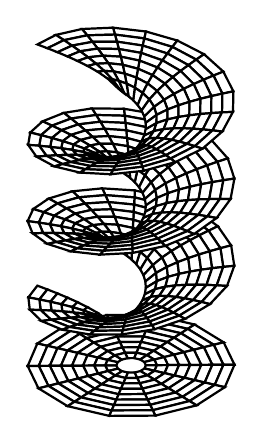
\begin{tikzpicture}[scale=2]
    \begin{axis}[
        axis lines=none,
        axis equal image,
        trig format plots=rad,
        z buffer=sort]
   \addplot3 [
        surf,
        domain=1:7,
        domain y=-pi:pi,
        samples=9,
        samples y=15,
        shader=flat,
        draw=black,
        fill=white
        ]
    ({x*cos(y)},{x*sin(y)},{-12});
   \addplot3 [
        surf,
        domain=1:7,
        samples=9,
        samples y=60,
        shader=flat,
        draw=black,
        fill=white,
        domain y=-3*pi:3*pi
        ]
    ({x*cos(y)},{x*sin(y)},{ln(x)+ y});
    \end{axis}
  \end{tikzpicture}



        This map \textit{should} be local homeomorphism, but this is false in the Zariski topology. There do not exist nonempty open subsets $V$ and $U$ such that $x \to x^n$ maps $V$ isomorphically onto $U$.
  \item fibre bundles aren't locally trivial.
\end{itemize}
  
These issues all stem from the fact that the Zariski topology is very coarse. Grothendieck found a natural generalisation of the notion of topology, allowing not only open subsets $U \subseteq X$ but more generally morphisms of schemes $Y \to X$ to play the role of open set. Specifically, he defined the \textit{\'etale site of $X$}, a generalised topology on $X$, consisting of the following:
\begin{itemize}
  \item The category of \'etale schemes $\text{\'Et}/X$ over $X$. This category consists of schemes $S$ together with an \'etale morphism $f: S \to X$. These morphisms formally behave like local homeomorphisms. 
  \item A notion of covering. In this case a covering of $X$ is a family of \'etale morphisms $\{\varphi_i: U_i \to X\}$ such that they are jointly surjective, $\bigcup_i im(\varphi_i) = X$. We will make this more precise later.
\end{itemize}
It will turn out that surjective \'etale maps are the right notion for a good covering theory for schemes. In particular they will allow us to define fundamental groups. Furthermore, the \'etale site will fix the issues we had in defining cohomology as well.

The \'etale topos $\mathsf{Sh}(X)$ of a scheme $X$ is the category of sheaves on the \'etale site of $X$.  The \'etale topos $\mathsf{Sh}(X)$ may be thought of as a generalised space, locally modeled on $X$, with a close relation to the geometric properties of $X$. 

Because \'etale morphisms behave like local homeomorphisms, it is possible to realise the theory of covering spaces for schemes. In particular this means that we get a good notion the fundamental groups $\pi_1(X)$. Furthermore, the \'etale topos $\mathsf{Sh}(X)$ also allows us to compute cohomology for sheaves which have vanishing cohomology in the Zariski setting. In this sense the \'etale site of a scheme is a much finer topology than the Zariski topology.


\section{Cohomology in Topology}
Cohomology is an important invariant in geometry and topology which associates to each space $X$ a sequence of abelian groups $H^i(X)$, $i \ge 0$, the so-called cohomology groups of $X$. For each map $f: X \to Y$ of spaces there are homomorphisms $f^*: H^i(Y) \to H^i(X)$. We can deduce many interesting properties of spaces from their cohomology groups and the associated homomorphisms.

Different notions of space, such as schemes, smooth manifolds and sheaves have properties that allow us to define cohomology which makes use of the particulars of this kind of space. Smooth manifolds, for instance, are topological spaces with additional “differentiable” structure. We may use this structure to define de Rham cohomology via differential forms.\\

There are theorems which relate these cohomology theories to each other.For example, de Rham's theorem states that the de Rham cohomology associated to smooth manifolds is isomorphic to singular cohomology with coefficients in $\mathbb{R}$. Another example of this is the fact that if $X$ is a locally contractible space, the singular cohomology $H_{\text{sing}}^i(X)$ of $X$ is isomorphic to the sheaf cohomology $H^i(X, \Z_X)$ of the constant sheaf $\Z_X$ on $X$. One of the main motivations for the \'etale topology and \'etale cohomology is that one would like a replacment for singular cohomology for schemes. For example, let $X$ be an irreducible scheme with generic point $\eta \in X$. Then $X$ is contractible, since $f: X \times I \to X$ defined by $f(x,0) = x$ and $f(x,t) = \eta$ for $t > 0$ is a contraction of $X$ to $\eta$.\\

A central tenent of geometry and topology is that in order to understand a space $X$, one may study functions $\varphi: X \to S$. Here, $S$ could be an algebraic structure or another space. Let us now consider for a moment the case $S=\mathbb{R}$. The simplest kind of functions are the constant ones. This does not yield any interesting information, as the set of constant functions into $\mathbb{R}$ is always isomorphic to $\mathbb{R}$. The second simplest case are locally constant functions. Let us denote the set of all locally constant functions from $X$ to $\mathbb{R}$ by $H^0(X,\mathbb{R})$. This set is a real vector space, whose dimension is the number of connected components of $X$. Cohomology

We briefly review some aspects of cohomology theory. This will serve as a model for what we expect of cohomology in the \'etale setting.

\subsection{Betti numbers and singular cohomology}
Betti numbers are invariants of topological spaces that, roughly speaking, quantify the number of ``holes'' that a topological space has in each dimension. For instance, the circle has 1 one-dimensional hole while the torus has 2. The sphere has 1 two-dimensional hole but no one-dimensional holes. 

We now provide a rigorous justification of this intuitive picture.

Let $X$ be a topological space and recall the definition of the standard simplices $\Delta^n$. The $\Hom$-functor $\Hom(\Delta^n, -)$ induces a simplicial set
\[\Sigma X: [n] \mapsto \Hom(\Delta^n, X).\]
A map $\sigma : \Delta^n \to X$ is called a singular $n$-simplex. One should think of $\Sigma X$ as a sort of triangulation of the space $X$. We now take for each $n$ the free abelian group $S_n(X)$ with basis $\Sigma X[n]$. An element $x$ of $S_n(X)$ is a formal linear combination $x = \sum_\sigma n_\sigma \sigma$ of $n$-simplices. 

%\subsection{De Rham Cohomology}
%
%An important version of cohomology arises from the theory of integration on manifolds. Stoke's theorem, Gauß's theorem and Green's theorem from analysis are all special cases of cohomological phenomena. The idea behind it is that the differential forms that can arise on a manifold are closely related to its topology. 
%
\subsection{The Mayer-Vietoris Sequence}

The Mayer-Vietoris sequence is an important tool for computing cohomology. It relates the cohomology of a space to the cohomology of its parts. To be more precise, suppose $U$ and $V$ are two subspaces of $X$ such that their interior covers $X$. Then, roughly speaking, there is an exact sequence

\[
\cdots \to H^n(X) \to H^n(U) \oplus  H^n(V) \to H^n(U\cap V) \to H^{n+1}(X) \to \cdots
\]

If the cohomology of $U$ and $V$ are known or easier to compute than the cohomology of$X$, this exact sequence provides a lot of information.

\subsection{Interpretation of Cohomology}
Cohomology groups are not just of interest in their own right. In many cases, one can show that the cohomology classes $[\gamma] \in H^n(X, \Sh{A})$ correspond bijectively to some other kind of geometrical construction involving $X$.

For instance, when $p:Z \to B$ is a map of topological spaces and $\Sh{G}$  is a sheaf of subgroups of $Aut_B(Z)$, one can define a notion of “twist of $p$ with structure sheaf $\Sh{G}$”. One obtains the bijection
\begin{align}
            \left\{ \parbox[c]{1.1in}{\centering
                       Isomorphism classes of twists of $p$
                       with structure sheaf $\Sh{G}$}
            \right\}
            \stackrel{\sim}{\to}
            \parbox[c]{0.5in}{\centering
                       $H^1(B, \Sh{G})$}
\end{align}

There is also a bijection
\begin{align}
            \left\{ \parbox[c]{1.1in}{\centering
              Isomorphism classes of vector bundles of rank $n$ with basis $B$}
            \right\}
            \stackrel{\sim}{\to}
            \parbox[c]{0.5in}{\centering
            $H^1(B, GL_{n,B})$}
\end{align}
and in particular
\begin{align}
            \left\{ \parbox[c]{1.1in}{\centering
            Isomorphism classes of line bundles with basis $B$}
            \right\}
            \stackrel{\sim}{\to}
            \parbox[c]{0.5in}{\centering
                $H^1(B, \Ring(O)_B^\times)$}
\end{align}

\subimport{introduction/}{mobius.tex}
\section{prerequisites}
We assume aqcuaintance with the basics of category theory including limits and adjoint functors. We will make free use of results from algebra but will provide references wherever needed. We will also use basic notions of scheme theory.

  \chapter{Simplicial Methods}
  \section{Simplicial Complexes}

Simplicial complexes are a generalization of directed graphs (among other things). They are widely used in algebraic topology because they provide a combinatorial model for "nice" topological spaces. Every covering $\mathcal{U}$ of a space $X$ gives rise to a simplicial complex $\mathcal{N(U)}$, the nerve of $\mathcal{U}$. The nerve theorem asserts that if a covering is "sufficiently nice", this simplicial complex is a good approximation for $X$, in the sense that $\mathcal{N(U)}$ presents the homotopy type of $X$.\\
Let $\mathcal{U} = \{U_\alpha\} = \{U_\alpha\}_{\alpha \in A}$ be a covering of a topological space or an object of a site $X$. For any finite set $l = \{a_0, \dots a_n\} \subseteq A$ we write $U_l$ or $U_{a_0 \cdots a_n}$ instead of $U_{a_0} \cap \cdots \cap U_{a_n}$ or $U_{a_0} \times_X \cdots \times_X U_{a_n}$.



\begin{theorem}[Nerve Theorem]
  Let $X$ be a paracompact space and $\mathcal{U}$ an open cover of $X$ such that every nonempty intersection of finitely many $U_i \in \mathcal{U}$ is contractible. Then $X$ is homotopy equivalent to $\mathcal{N(U)}$.
\end{theorem}
\begin{proof}
  By a previous lemma. %4.G.2 in Hatcher, will try to a implement

\end{proof}

  \chapter{Cohomology in Topology}
  \label{chap:cohomology}
  Cohomology is an important invariant in geometry and topology. It is a tool which associates to each space $X$ a sequence of abelian groups $H^i(X)$, $i \ge 0$, the so-called cohomology groups of $X$. For each map $f: X \to Y$ of spaces there are homomorphisms $f^*: H^i(Y) \to H^i(X)$. We can deduce many interesting properties of spaces from their cohomology groups and the associated homomorphisms.

Various notions of space, such as schemes, smooth manifolds and sheaves have properties that allow us to define cohomology which makes use of the particulars of this kind of space. Smooth manifolds, for instance, are topological spaces with additional “differentiable” structure.  We may use this structure to define de Rham cohomology via differential forms.

This section will give an overview of some important cohomology theories to indicate their importance in geometry, but we will not be proving any theorems.
We will see theorems which relate these cohomology theories to each other so that we may often choose an appropriate method for computation. For example, de Rham's theorem states that the de Rham cohomology associated to smooth manifolds is isomorphic to singular cohomology with coefficients in $\mathbb{R}$. 

A central tenent of geometry and topology is that in order to understand a space $X$, one may study functions $\varphi: X \to S$. Here, $S$ could be an algebraic structure or another space. Let us now consider for a moment the case $S=\mathbb{R}$. The simplest kind of functions are the constant ones. This does not yield any interesting information, as the set of constant functions into $\mathbb{R}$ is always isomorphic to $\mathbb{R}$. The second simplest case are locally constant functions. Let us denote the set of all locally constant functios from $X$ to $\mathbb{R}$ by $H^0(X,\mathbb{R})$. This set is a real vector space, whose dimension is the number of connected components of $X$. In the section on de Rham cohomology we will define higher dimensional analogues $H^i_{dR}(X)$ of this vector space.

Another central notion of modern geometry is that one thinks of spaces as being “glued together” from simple building blocks. A manifold is locally modelled on $\mathbb{R}^n$. A simplicial complex and more generally simplicial sets and simplicial objects are geometric objects that are modeled on the standard simplices $\Delta^n$, depicted below for $n = 1,2,3$.

\section{De Rham Cohomology}

An important version of cohomology arises from the theory of integration on manifolds. Stoke's theorem, Gauß's theorem and Green's theorem are all special cases of cohomological phenomena.

\section{The Mayer-Vietoris Sequence}

The Mayer-Vietoris sequence is an important tool for computing cohomology. It relates the cohomology of a space to the cohomology of its parts. To be more precise, suppose $U$ and $V$ are two subspaces of $X$ such that their interior covers $X$. Then, roughly speaking, there is an exact sequence

$$
\cdots \to H^n(X) \to H^n(U) \oplus  H^n(V) \to H^n(U\cap V) \to H^{n+1}(X) \to \cdots      
$$

If the cohomology of $U$ and $V$ are known or easier to compute than the cohomology of$X$, this exact sequence provides a lot of information.


Cohomology groups are not just of interest in their own right. In many cases, one can show that the cohomology classes $[\gamma] \in H^n(X, \mathcal{A})$ correspond bijectively to some other kind of geometrical construction involving $X$.

For instance, when $p:Z \to B$ is a map of topological spaces and $\mathcal{G}$  is a sheaf of subgroups of $Aut_B(Z)$, one can define a notion of “twist of $p$ with structure sheaf $\mathcal{G}$”. One obtains the bijection
\begin{align}
            \left\{ \parbox[c]{1.1in}{\centering
                       Isomorphism classes of twists of $p$
                       with structure sheaf $\mathcal{G}$}
            \right\}
            \stackrel{\sim}{\longrightarrow}
            \parbox[c]{0.5in}{\centering
                       $H^1(B, \mathcal{G})$}
\end{align}

There is also a bijection
\begin{align}
            \left\{ \parbox[c]{1.1in}{\centering
              Isomorphism classes of vector bundles of rank $n$ with basis $B$}
            \right\}
            \stackrel{\sim}{\longrightarrow}
            \parbox[c]{0.5in}{\centering
            $H^1(B, GL_{n,B})$}
\end{align}
and in particular
\begin{align}
            \left\{ \parbox[c]{1.1in}{\centering
            Isomorphism classes of line bundles with basis $B$}
            \right\}
            \stackrel{\sim}{\longrightarrow}
            \parbox[c]{0.5in}{\centering
                $H^1(B, \mathcal{O}_B^\times)$}
\end{align}

To get a first taste of cohomology we consider a directed graph $X$. The set of all functions from the set of vertices of $X$to $\mathbb{Z}$ is an abelian group by pointwise addition. We will denote this group by $C^1_*(X)$ and call it the group of $1$-cochains. Likewise there is a group $C^2_*(X)$, consisting of functions from the edges of $X$ to $\mathbb{Z}$. We can interpret the vertices of $X$ to lie on a map, and an element $\varphi \in C^1_*(X)$ to assign an elevation to each vertex. There is then a natural map


  \chapter{Sites and Sheaves}
  Much of modern geometry can be formulated in the language of sheaves. Sheaves are data that are given on a topological space that may be glued. One may more generally define sheaves on a category equipped with a so-called Grothendieck topology.

\begin{construction}\label{def:opens}
  Let $X$ be a topological space. The open sets of $X$ are partially ordered by inclusion: \[V \le W \quad \text{iff} \quad V \subseteq W.\]
  We may thus consider the category of open sets of $X$, denoted by $\Op(X)$.
\end{construction}
A key observation is the following: In the category $\Op(X)$ pullbacks correspond to intersections and pushouts correspond to unions. By the definition of topological space, this means that $\Op(X)$ has finite pullbacks and arbitrary pushouts.

\begin{definition}[Presheaves] 
  Let $X$ be a topological space. A \textit{presheaf of sets} $\mathcal{F}$  is a map which assings
  \begin{enumerate}
    \item to each open subset $U$ of $X$ a set $\mathcal{F}(U)$. We call the elements of $\mathcal{F}(U)$ the \textit{sections of $\mathcal{F}$ over $U$}.
    \item to each inclusion of open sets $U \subseteq V$ a \textit{restriction map}
    \[res_{V\kern-0.1em , U}: \mathcal{F}(V) \longrightarrow\mathcal{F}(U).\]
  \end{enumerate}
    The restriction maps need to have the following properties: 
    \begin{enumerate}
      \item The restriction along the identity $V \subseteq V$ is the identity, so 
            \[res_{V\kern-0.1em , V} = id.\]
      \item For two inclusions $U \subseteq V \subseteq W$, the restricion maps adhere to the identity 
            \[res_{W\kern-0.1em , V}\ \circ\ res_{V\kern-0.1em , U} = res_{W\kern-0.1em , U}.\]
    \end{enumerate}
  One may more slickly define a presheaf as a functor $\mathcal{F}: \Op(X)^{\op}\longrightarrow \Set$. To supress notation we will write $s|_V$ instead of $res_{V\kern-0.1em , U}(s).$ Here $s$ is a section over $U$.\\
\end{definition}
\begin{definition}[Sheaves]
  A presheaf $\mathcal{F}$ is a \textit{sheaf} if one can uniquely glue sections. Precisely, this means:
  \begin{enumerate}
    \item For an open set $U$, an open cover $\{U_i\}_{\indexset{i}{I}}$ of $U$ and $s, t \in \mathcal{F}(U)$, if $s|_{U_i} = t|_{U_i}$ for all $i \in I$, then $s = t$.
    \item For an open set $U$, an open cover $\{U_i\}_{\indexset{i}{I}}$ of $U$ and a family of sections
    \[\{s_i \in \mathcal{F}(U_i)\}_{\indexset{i}{I}},\]
     if $s_i|_{U_i \cap U_j} = s_j|_{U_i \cap U_j}$ for all $i,j \in I$, then there exists a section $s \in \mathcal{F}(U)$ such that $s|_{U_i} = s_i$ for all $i \in I$.
  \end{enumerate}
  In words this says that if we have a a cover $\{U_i\}$ of $U$ and a family of sections $\{s_i\}$ which agree on all intersections, we may glue these sections to a section over $U$. Moreover, this section is unique.
\end{definition}

% TODO: Examples: constant sheaves, sheaves of rings
The definition for presheaves and sheaves are given almost entirely in categorical language. The notion of presheaf on a category $C$ is readily defined as a functor 
\[\mathcal{F}: C^{\op}\longrightarrow \Set.\]
What is required for the definition of sheaves to work is the notion of covering in a category. To motivate the definition of a Grothendieck topology, we review the proerties of coverings in the language introduced in Definition \ref{def:opens}.
 \begin{enumerate}
  \item The identity $U \to U$ is an open cover of $U$.
  \item Coverings are stable under composition. Precisely this means: Given a covering \\$\{U_i \to U\}_{i \in I}$ and for each $U_i$ a covering $\{V_{ij} \to U_i\}_{j \in J}$, the composition
        \[\{V_{ij} \to U\}\]
        should be a covering of $U$.
   \item  Coverings are stable under pullback: If we have an inclusion $V \hookrightarrow U$ and a covering $\{U_i \to U\}$, the open sets $\{U_i \times_U V\}$ cover $V$ with the induced projection maps:
   % https://q.uiver.app/?q=WzAsNCxbMCwwLCJcXHtVX2kgXFx0aW1lc19VIFZcXH0iXSxbMCwxLCJWIl0sWzEsMCwiXFx7VV9pXFx9Il0sWzEsMSwiVSJdLFswLDFdLFswLDJdLFsyLDNdLFsxLDMsIiIsMCx7InN0eWxlIjp7InRhaWwiOnsibmFtZSI6Imhvb2siLCJzaWRlIjoidG9wIn19fV1d
      \[\begin{tikzcd}
      	{\{U_i \times_U V\}} & {\{U_i\}} \\
      	V & U.
      	\arrow[from=1-1, to=2-1]
      	\arrow[from=1-1, to=1-2]
      	\arrow[from=1-2, to=2-2]
      	\arrow[hook, from=2-1, to=2-2]
      \end{tikzcd}\]
      Here the fiber product is to be interpreted as the intersection.
\end{enumerate}
\begin{definition}[bases for Grothendieck topologies]
  
\end{definition}

\begin{definition}[the atomic site]

\end{definition}
The atomic site is subcaonical if and only if every morphism in the category is a regular epimorphism. This means that every morphism is the coequalizer of some parallel pair of morphisms.

Taken from \cite{barr/diaconescu:1980}. \\
Fix a perfect field $k$. We denote by $k_{Ext}$ the category of separable field extensions of $k$. If $L_1$ and $L_2$ are two extensions of $k$, then $L_1 \otimes_k L_2$ is a product of a finite number of separable extensions of $k$. Thus $k_{Ext}$ is dual to an atomic site. A sheaf on this site is given by a morphism of sites $f\colon k_{Ext}^{\op} \longrightarrow \Set$. This is just a presheaf on $k_{Ext}$, and is thus a colimit of representables $f(K) = \colim(K, K_i)$. ...\\

  \chapter{\'Etale Cohomology}
  A locally ringed space $(X, \OO_X)$ is a topological space $X$ together with a sheaf of rings $\OO_X$, such that all stalks $\colim \OO_X(X)$.
%A scheme is in particular a locally ringed space, meaning it comes equipped with a sheaf of rings such that the stalks are local rings. This has some important consequences for the theory of schemes. If we wish to take seriously the \'etale topology as a replacement for the Zariski topology, these consequences should have analogues in the \'etale setting as well.
%
%For a sheaf of rings $\mathcal{F}$, the stalk of $\mathcal{F}$ at $x \in X$ is defined to be $\colim F(U)$, where $U$ runs over all neighborhoods of $x$. This group captures the local behavior of $\mathcal{F}$ around $x$. For this definition to make sense in the \'etale setting, we need to verify that the category of \'etale neighborhoods at $x$ is cofiltered.k
%
%\section{A brief Reminder on Schemes}
%The starting point of modern algebraic geometry is the definition of affine schemes. We briefly recall the definition and its most important consequences, after which we will construct their analogues in the \'etale setting.
%
%Let $A$ be a ring. The spectrum of $A$ is the set $\{\mathfrak{p} \subseteq A | \mathfrak{p} \text{ prime ideal}\}$. For any ideal $\mathfrak{a}$ of $A$ we write $V(\mathfrak{a})$ for the set of prime ideals containing $\mathfrak{a}$. By basic algebra one may deduce that the sets $V(\mathfrak{a})$ form the closed sets of a topology on $\Spec A$. 
%%Affine schemes are locally ringed spaces constructed from commutative rings. We briefly recall the construction. Let $A$ be a commutative ring. We put a topology on the set of prime ideals of $A$. 
%%$\{\mathfrak{p} \subseteq A | \mathfrak{p} \text{ prime }\}$
%
%
%Schemes are locally ringed spaces that are locally affine.
%Now that we have available the \'etale topology for a scheme
  The issues we encountered in the introduction all stem from the fact that the Zariski topology is very coarse. Grothendieck found a natural generalisation of the notion of topology, allowing not only open subsets $U \subseteq X$ but more generally morphisms of schemes $Y \to X$ to play the role of open set. Specifically, he defined the \textit{\'etale site of $X$}, a generalised topology on $X$, consisting of the following:

\begin{itemize}
  \item The category of \'etale schemes $\text{\'Et}/X$ over $X$. This category consists of schemes $S$ together with an \'etale morphism $f: S \to X$. These morphisms formally behave like local homeomorphisms. 
  \item A notion of covering. In this case a covering of $X$ is a family of \'etale morphisms $\{\varphi_i: U_i \to X\}$ such that they are jointly surjective, $\bigcup_i im(\varphi_i) = X$. 
\end{itemize}

In this section we will define and study \'etale morphisms.  Because \'etale morphisms behave like local homeomorphisms, it is possible to realise the theory of covering spaces for schemes. In particular this means that we get a good notion the fundamental groups $\pi_1(X)$. The definition of a sheaf carries over seamlessly from the classical case of topological spaces to the case of sheaves on sites. The \'etale topos $\mathsf{Sh}(X)$ of a scheme $X$ is the category of sheaves on the \'etale site of $X$.  The \'etale topos of $X$ may be thought of as a generalised space, locally modeled on $X$, with a close relation to the geometric properties of $X$.  Furthermore, the \'etale topos $\mathsf{Sh}(X)$ also allows us to compute cohomology for sheaves which have vanishing cohomology in the Zariski setting. In this sense the \'etale site of a scheme is a much finer topology than the Zariski topology.

\subsection{\'Etale Algebras}
We begin our discussion with the simple case of \'etale covers of $X = \Spec(k)$, where $k$ is a field. In order to model the notion of local homeomorphism, it is reasonable to demand that for $f: Y \to \Spec(k)$ to be a local homeomorphism,  the underlying topological space of $Y$ should consist of a finite number of disjoint points. If we restrict our attention to the case that $Y$ is affine, it follows that $Y = \Spec(\prod L_i)$ where each $L_i$ is a field extension of $k$. 

\begin{definition}[finite \'etale algebras]
  A finite dimensional $k$-algebra $A$ is \'etale over $k$ if it is isomorphic to a product of separable extensions of $k$. We define $\Spec(A) \to \Spec(k)$ to be \'etale if $A$ is an \'etale algebra over $k$.
\end{definition}

Recall that an extension $L/k$ is separable if its minimal polynomial $p(x)$ has no multiple roots (in a splitting field of $p(x)$). It follows from basic algebra that a polynomial $p(x)$ is separable if and only if it is coprime to its derivative $p'(x)$. This means that $p'(x)$ gets mapped to a unit under the canonical map $k[x] \to k[x]/(p(x)) \simeq L$. This is in effect a smoothness condition, reminiscent of the conditions under which the inverse mapping theorem from analysis holds. This idea will reappear when we define \'etale morphisms in a more general condition.

\subsubsection{Galois theory for finite \'etale algebras}
We recall the basics of Galois theory as Grothendieck formulated them.

\begin{construction}[Reminder on Galois theory]
  Let $k$ be a field and fix once and for all separable and algebraic closures $k_s \subset \overline{k}$.  An algebraic extension $L$ of $k$ is a \textit{Galois extension} if the elements of $L$ that are fixed under the automorphism group $\Aut_k(L)$ are precisely the elements of $k$. In this case we call $\Aut_k(L)$ the \textit{Galois group} of $L$ over $k$ and denote it by $\Gal(L/k)$. A separable extension $L/k$ is Galois if and only if the minimal polynomial of each element $a \in L$ splits into linear factors in $L$. In particular $k_s$ is a Galois extension. We call its Galois grouop the \textit{absolute Galois group of $k$} and denote it by $\Gal(k)$. If $k_s$ is an infinte extension, $\Gal(k)$ is a profinite group and hence carries a totally disconnected topology. Let $L$ be a finite separable extension of $k$. The set $\Hom_k(L, k_s)$ is finite and equal to $[L:k]$. This set is endowed with a left action of $\Gal(k_s/k)$ given by $\varphi \to g \circ \varphi$ for $g \in \Gal(k)$ and $\varphi \in \Hom_k(L, k_s)$. The action of $\Gal(k)$ is continuous if $\Hom(L, k_s)$ is given the discrete topology. In this case, we can verify continuity by checking that each stabilizer 
  \[G_x = \{ g \in G \mid g \circ \varphi =  \varphi \forall\ \varphi \in \Hom_k(L, k_s)\}, \]
  which is easy to check.
\end{construction}

\begin{proposition}
  The action of $\Gal(k)$ on $\Hom_k(L, k_s)$ is continuous and transitive and $\Hom_k(L, k_s)$ is isomorphic as a left $\Gal(k)$-set to the $\Gal(k)$-set $G/U$ for some open subgroup $U \subseteq \Gal(k)$
\end{proposition}

\begin{theorem}[Main Theorem of Galois Theory, Grothendieck's version]
  Let $k$ be a field. The functor mapping a finite \'etale $k$-algebra $A$ to the finite set $\Hom_k(A, k_s)$ induces an equivalence of categories between the cateogry of finite \'etale $k$-algebras and the category of finite sets with a continous left $\text{Gal}(k)$-action.
\end{theorem}

This theorem is strongly reminiscent of the following theorem from algebraic topology:

\begin{theorem}
  Let $(X,x)$ be a pointed, connected and locally simply connected topological space. The fiber functor $\text{Fib}_x$ induces an equivalence of categories between the category of covers of $X$ with the category of left $\pi_1(X,x)$-sets.
\end{theorem}

See Chapter (...) for the definitions used in the statement.

Let $L/K$ be a finite field extension of degree $n$. Each element $a$ of $L$ induces a $K$-linear map 
\[
  m_a: L \to L,\ b \to ab.
\]
Since $L \cong K^{\oplus n}$ as a $K$-module, we may choose a basis of $L$ over $K$ and represent the map $m_a$ as an $n \times n$ matrix with entries in $K$. We may take the trace and determinant of this matrix. But the trace and determinant are independent of the choice of the choice of basis, so
\[ 
  \Tr_{L/K}(a) = \Tr(\text{matrix of }m_a)
\]
and
\[ 
  \Norm_{L/K}(a) = \text{det}(\text{matrix of }m_a).
\]
are well defined.

\begin{definition}
  Let $L/K$ be a finite field extension. The \textit{trace pairing for $L/K$} is the symmetric $K$-bilinear form
  \[
    Q_{L/K} : L \times L \to K,\ (a,b) \to \Tr_{L/K}(ab)
  \]
\end{definition}

\begin{lemma}
  Let $L/K$ be a finite field extension. The following are equivalent:
  \begin{enumerate}
    \item $L/K$ is separable.
    \item $\Tr_{L/K}$ is not identically zero.
    \item $Q_{L/K}$ is nondegenerate.
  \end{enumerate}
\end{lemma}

\begin{proof}
  The equivalence of (2.) and (3.) are clear. 
  For the equivalence of (1.) and (2.) see (Keith Conrad, separability)
  %The trace map is $K$-linear with target $K$ so it is either  identically 0 or surjective.  We only have to consider the case where $K$ has characteristic $p \neq 0$, since finite extensions in characteristic 0 are always separable and $\Tr_{L/K}(1) = [L:K] \neq 0$ in characteristic 0.\par
  %Let $L/K$ be separable. By the primitive element theorem we can write $L = K(\alpha)$, where $\alpha$ is separable over $K$.
\end{proof}

\begin{theorem}
  Let $A$ be a finite dimensional commutative $k$-algebra and denote by $\overline{A}$ the $\overline{k}$-algebra $A \otimes_k \overline{k}$. The following are equivalent:
  \begin{enumerate}
    \item $A$ is \'etale over $k$.\label{etale}
    \item $A \otimes_k \overline{k}$ is isomorphic to a finite product of copies of $\overline{k}$, hence \'etale over $\overline{k}$.\label{product}
    \item $A \otimes_k \overline{k}$ is reduced
    \item The discriminant of any basis of $A$ over $k$ is nonzero.\label{trace}
    %The trace pairing $A \times A \to k, (x,y) \to \text{Tr}(xy)$ is nondegenerate.
  \end{enumerate}
\end{theorem}

\begin{proof}
  (\Implies{etale}{product}):
  Suppose that $L$ is a finite separable extension of $k$. This means that $L = k[x]/(f)$, where $f$ is a polynomial of degree $n$ which splits into $n$ distinct factors, say $(x-\alpha_i)$ in $\overline{k}$. By the chinese remainder theorem we have
  \[L \otimes_k \overline{k} \cong \overline{k}[x]/(f) = \overline{k}[x]/(x-\alpha_1)\cdots(x-\alpha_n) \cong \prod_{i=1}^n \overline{k}[x] / (x-\alpha_i) \cong \prod_{i=1}^n \overline{k},\] from which the first direction follows.\\
  (\Implies{etale}{trace}):
  If $A = \prod k_i$  where each $k_i$ is a separable field extension of $k$, then $\text{disc}(A) = \prod \text{disc}(k_i)$ which is nonzero by the fact that $\text{disc}(k_i) \neq 0$ if $k_i$ is a separable extension.
  %TODO finish the proof
\end{proof}

We generalise the notion of \'etale algebra to algebras over a ring.

\begin{definition}
  Let $R$ be a ring, $A$ a free $R$-algebra of finite rank. As before, every $a \in A$ defines an $R$-linear map by multiplication and the trace map $A \to R$ is well defined. We say that $A$ is a \textit{separable} or \textit{\'etale} algebra if the $R$-bilinear mapping 
  \[
    Q : A \times A \to R,\ (a,b) \to \Tr(ab)
  \]
  is nondegenerate.
\end{definition}

\subsection{\'Etale morphisms of schemes}
\begin{definition}
A morphism of schemes $f: X \to Y$ is called \textit{affine} if there is an open affine cover by subsets $U_i$ such that $f^{-1}(U_i)$ is affine for each $i$.  A morphism of schemes $f: X \to Y$ is called \textit{finite} if there is an affine cover by subsets $U_i = \Spec(A)$ such that $f^{-1}(U_i) = \Spec(B_i)$ is a finitely generated $A_i$-module.  If moreover each $B_i$ is a fee separable $A_i$-algebra, it is said to be \'etale.
%We say that $f: X \to S$ is finite locally free if $f$ is affine and $f_* \Sh{O}_X$ is locally free and of finite rank.
%If each fibre $X_p$ of $f$ is the spectrum of a finite \'etale $\kappa(p)$-algebra, then we say $f$ is an \'etale morphism.
\end{definition}
It follows that $f: \Spec(B) \to \Spec(A)$ is an \'etale morphism if and only if $B$ is an \'etale $A$-algebra.

\begin{lemma}
  \begin{enumerate}
    \item The composition of affine morphisms is affine.
    \item The composition of finite locally free morphisms is finite locally free.
    \item The composition of \'etale morphisms is \'etale.
  \end{enumerate}
\end{lemma}
\begin{proof}
  The first statement follows immediately from the fact that a morphism $f: X \to Y$ is affine if and only if for \textit{every} affine open $V \subseteq X$, $f^{-1}(V)$ is affine, see\cite{Hartshorne}.
\end{proof}


\begin{lemma}
  If $f: Y \to X$ is \'etale, then the base change $U \times_X Y$ along any morphism $U \to X$ is \'etale.
\end{lemma}
\begin{definition}
  A surjective finite \'etale morphism is called an \'etale cover. An \'etale cover $\varphi : Y \to X$ is claled trivial if $Y$ is isomorphic do a finite disjoint union of copies of $X$ $Y \cong \coprod X$ and $\varphi$ restricts to the identity on each component.
\end{definition}

\begin{theorem} 
  \label{locallyTrivial}
  Let $X$ be a connected scheme and $\varphi : Y \to X$ an affine surjective morphism. Then $\varphi$ is finite \'etale if and only if there is a finite, locally free and surjective morphism $f: S \to X$ such that $Y \times_X S$ is a trivial cover of $S$.
\end{theorem}
\begin{proof}
  $(\implies)$
  We first show that $\varphi$ is finite and locally free. Since $f$ is locally free, each point of $X$ has an affine open neighborhood $U = \Spec(R)$ such that $f$ restricts to a morphism $\Spec(A) \to \Spec(R)$ where $A$ is a finitely generated and free $R$-module. Since $\varphi$ is affine, it restricts to $\Spec(B) \to \Spec(R)$ over $U$ and the basechange $S \times_X Y$ restricts to $\Spec(A \otimes_R B)$ over $\Spec(R)$. By assumption $A \otimes_R B$ is a finitely generated and free $A$-module, so it is also fnitely generated and free as an $R$-module. It is also isomorphic to a finite direct sum of copies of $A$. This can only happen if $B$ is finitely generated and free over $R$.
    \[
    % https://q.uiver.app/?q=WzAsOCxbMCwxLCJTIl0sWzEsMCwiWSJdLFsxLDEsIlgiXSxbMCwwLCJTIFxcdGltZXNfWCBZIl0sWzIsMCwiXFxTcGVjKEEgXFxvdGltZXNfUkIpIl0sWzIsMSwiXFxTcGVjKEEpIl0sWzMsMSwiXFxTcGVjKFIpIl0sWzMsMCwiXFxTcGVjKEIpIl0sWzEsMiwiXFx2YXJwaGkiXSxbMCwyLCJmIiwyXSxbMywxXSxbMywwXSxbNCw1XSxbNSw2XSxbNCw3XSxbNyw2XV0=
    \begin{tikzcd}
    	{S \times_X Y} & Y & {\Spec(A \otimes_RB)} & {\Spec(B)} \\
    	S & X & {\Spec(A)} & {\Spec(R)}
    	\arrow["\varphi", from=1-2, to=2-2]
    	\arrow["f"', from=2-1, to=2-2]
    	\arrow[from=1-1, to=1-2]
    	\arrow[from=1-1, to=2-1]
    	\arrow[from=1-3, to=2-3]
    	\arrow[from=2-3, to=2-4]
    	\arrow[from=1-3, to=1-4]
    	\arrow[from=1-4, to=2-4]
    \end{tikzcd}
    \]
  Now let $\overline{x} : \Spec(\overline{k}) \to S$ be a geometric point of $S$. By composition with $f$ we get a geometric point of $X$. Now the geometric fibers $Y_{(f \circ \overline{x})}$ and $(S \times_X Y)_{\overline{x}}$  are isomorphic by the universal property of pullbacks. 
  \[
  % https://q.uiver.app/?q=WzAsOSxbMiwxLCJYIl0sWzIsMCwiWSJdLFsxLDAsIllfeyhmIFxcY2lyYyBcXG92ZXJsaW5le3h9KX0iXSxbMSwxLCJcXG92ZXJsaW5le2t9Il0sWzMsMCwiKFMgXFx0aW1lc19YIFkpX3tcXG92ZXJsaW5le3h9fSJdLFszLDEsIlxcb3ZlcmxpbmV7a30iXSxbNCwwLCJTIFxcdGltZXNfWCBZIl0sWzQsMSwiUyJdLFswLDJdLFsxLDBdLFsyLDFdLFszLDAsImYgXFxjaXJjIFxcb3ZlcmxpbmV7eH0iLDJdLFsyLDNdLFs0LDVdLFs0LDZdLFs2LDddLFs1LDcsIlxcb3ZlcmxpbmV7eH0iLDJdXQ==
\begin{tikzcd}
	& {Y_{(f \circ \overline{x})}} & Y & {(S \times_X Y)_{\overline{x}}} & {S \times_X Y} \\
	& {\overline{k}} & X & {\overline{k}} & S \\
	{}
	\arrow[from=1-3, to=2-3]
	\arrow[from=1-2, to=1-3]
	\arrow["{f \circ \overline{x}}"', from=2-2, to=2-3]
	\arrow[from=1-2, to=2-2]
	\arrow[from=1-4, to=2-4]
	\arrow[from=1-4, to=1-5]
	\arrow[from=1-5, to=2-5]
	\arrow["{\overline{x}}"', from=2-4, to=2-5]
\end{tikzcd}
\]
By assumption, $(S\times_X Y)_{\overline{x}} \cong \prod \Spec(\overline{k})$ and since $f$ is surjective, all of the fibers of $\varphi$ are also \'etale.
\end{proof}
Theorem \ref{locallyTrivial} shows that \'etale morphsism are locally trivial in the \'etale topology.

\begin{remark}
  If we have an \'etale cover $f: Y \to X$ and consider a geometric point $\overline{x} : \Spec(\Omega) \to X$ of $X$, then the fiber of $f$ over $\overline{x}$ arises from the pullback
    % https://q.uiver.app/?q=WzAsNCxbMCwwLCJTcGVjKFxcT21lZ2EpXFx0aW1lc19YIFkiXSxbMCwxLCJTcGVjKFxcT21lZ2EpIl0sWzEsMCwiWSJdLFsxLDEsIlgiXSxbMCwxXSxbMCwyXSxbMiwzXSxbMSwzXV0=
    \[\begin{tikzcd}
    	{\Spec(\Omega)\times_X Y} & Y \\
    	{\Spec(\Omega)} & X
    	\arrow[from=1-1, to=2-1]
    	\arrow[from=1-1, to=1-2]
    	\arrow[from=1-2, to=2-2]
    	\arrow[from=2-1, to=2-2]
    \end{tikzcd}\]
  Since $\Spec(\Omega)\times_X Y$ is \'etale over $\Spec(\Omega)$ and $\Omega$ is algebraically closed, it follows that $\Spec(\Omega)\times_X Y \cong \coprod \Spec(\Omega)$.
\end{remark}

\subsection{Galois theory for \'etale covers}
\begin{definition}[The fiber functor $F_x$]
  Let $x: \Spec(\Omega) \to X$ be a geometric point, where $\Omega$ is an algebraically field. The fiber functor at $x$ associates to each \'etale cover $f: Y \to X$ the underlying set of $\Spec(\Omega) \times_X Y$.
\end{definition}

\begin{remark}
  In topology, the fiber functor is representable if $X$ is a connected and locally simply connected space. The representing object $\tilde{X}$ is called the universal covering. In algebraic geometry this functor is usually not representable. It is however pro-representable:
\end{remark}

\begin{definition}[Pro-representability]
  Let $C$ be a category and $F: C \to \Set$ a functor. We say that $F$ is \textit{pro-representable} if there exists an \Gls{inverse system} $(A_\alpha,\varphi_{\alpha \beta})$ in $C$ such that 
  \[
    \varinjlim \Hom(A_\alpha, X) \cong F(X)
    \]
  for each $X$ in $C$.
\end{definition}
\begin{lemma}
  Let $f: Y \to X$ be a connected finite \'etale cover. There is a morphism $\varphi: S \to Y$ such that $f \circ \varphi: S \to X$ is a finite \'etale cover. Moreover every morphism over $X$ from a Galois cover to $Y$ factors through $\varphi$.
\end{lemma}

\begin{theorem}\label{thm:pro_rep}
  The fiber functor $F_{\overline{x}}$ is prorepresentable.
\end{theorem}
\begin{proof}[Proof of theorem \ref{thm:pro_rep}]
  We need to construct an inverse system in $Fet/X$ such that the above isomorphism holds. Take as index set $I$ all finite \'etale Galois covers $A_\alpha$ of $X$. This set is directed under the order $A_\alpha \le A_\beta$, since the connected components fiber product
\end{proof}

\begin{theorem}
  Let $X$ be a scheme and $\overline{x} : \Spec(\Omega) \to X$ a geometric point.
\end{theorem}

\begin{definition}[Galois covers]
  A connected finite \'etale cover $Y \to X$ is \textit{Galois} if its group of $X$-automorphism acts transitively on geometric fibers.
\end{definition}


\begin{definition}[Affine maps of schemes]
  Let $\varphi: X \to Y$ be a morphism of schemes over a field $k$. We say $\varphi$ is an affine map if every open affine subscheme $U = \Spec(R) \subseteq Y$ has as preimage an affine open subscheme $f^{-1}(U) = \Spec(S)$ of $X$. If, in addition, the corresponding map $R \to S$ makes $S$ into a finitely generated $R$-module, we say that $\varphi$ is finite.
\end{definition}

\begin{proposition}
Let $k$ be a field. Then $X$ is finite \'etale over $\Spec(k)$ if and only f $X$ is isomorphic to a disjoint union $\amalg \Spec(K_i)$, where each $K_i$ is a finite separable extension of $k$
\end{proposition}
\begin{proof}
  Consider first the case that $X$ is connected. It follows that $X = \Spec(A)$ and that $A$ is a vector space of finite dimension over $k$. If $A$ is not a field then it has a
\end{proof}



\begin{definition}[Faithfully flat morphisms]
   An $R$-module $M$ is \textit{flat} if the functor $N \to M \otimes_R M$ is exact. In other words: tensoring with $M$ preserves exact sequences. If the functor is also faithful, we say that $M$ is \textit{faithfully flat} over $R$.
\end{definition}

%
%\section{The \'Etale Fundamental Group}
%\subsection{The Fundamental Group in Topology}
%\subsection{Classical Galois Theory}
%Recall the main theorem of classical Galois theory:
%\begin{theorem}[Main Theorem of Galois theory for finite extensions]
%  Let $L/k$ be a finite Galois extension with Galois group $G$. There is an inclusion reversing bijection between subextension $ L \supset M \supset k$ and subgroups $H \subset G$. It is given by the maps
%  \begin{align*}
%    M &\mapsto \text{Aut}(L/M) \\
%    H &\mapsto L^H.
%  \end{align*}
%  %missing some explanation
%\end{theorem}
%This theorem fails for infinite Galois extensions, as the following example shows:
%% missing example
%

  \chapter{\'Etale Homotopy}

  \chapter{Conclusion}
  \input{chapters/conclusion}

  \bibliographystyle{plain}
  \bibliography{refs}
\end{document}